% =============================================================================
% KAPITEL 8 – Evaluation der entwickelten Strategie (GEKÜRZT)
% =============================================================================

\chapter{Evaluation der entwickelten Strategie}

Das vorliegende Kapitel prüft, inwieweit die in Kapitel~6 konzipierte und in Kapitel~7 prototypisch umgesetzte Observability-Strategie die Anforderungen aus Kapitel~3 erfüllt.


\section{Evaluationsmethodik}

Die Evaluation folgt dem in Abschnitt~4.3 definierten Bewertungsrahmen mit drei Evidenzquellen: Artefaktanalyse, Konfigurations- und Instrumentierungsprüfung sowie Last- und Störungsszenarien. Im Prototyp (Kapitel~7) wurden die ersten beiden Quellen ausgeschöpft. Die dritte blieb auf manuelle Plausibilitätstests beschränkt. Um diese Lücke zu verkleinern, wurden drei gezielte Belastungsszenarien auf dem Staging-Server durchgeführt: CPU-Last auf dem Backend-Container für den Latenz-Alert, temporäre Unterbrechung der Datenbankverbindung für den Fehler-Alert und Erschöpfung des PostgreSQL-Verbindungspools für den Sättigungs-Alert. Ergänzend wurde die bidirektionale Log-Trace-Korrelation auf dem Staging-Server verifiziert.


\section{Anforderungsbezogene Bewertung}

Tabelle~\ref{tab:eval-synthese} gibt vorab einen kompakten Überblick über die Erfüllungsgrade. Die folgenden Unterabschnitte begründen diese Einstufungen.

\begin{table}[htb]
\centering
\caption[Ergebnissynthese der anforderungsbezogenen Evaluation.]{Ergebnissynthese der anforderungsbezogenen Evaluation. \small Quelle: Eigene Darstellung.}
\label{tab:eval-synthese}
\small
\begin{tabularx}{\textwidth}{l >{\RaggedRight\arraybackslash}X >{\RaggedRight\arraybackslash}X l}
\toprule
\textbf{Anf.} & \textbf{Kurzbefund} & \textbf{Wesentliche Einschränkung} & \textbf{Erfüllungsgrad} \\
\midrule
A1 & Backend-Pfad rekonstruierbar, Gesamtsystem unvollständig & AI Provider und Frontend nicht instrumentiert & teilweise erfüllt \\[4pt]
A2 & Drei Messebenen für instrumentierte Dienste vorhanden & Keine Browser-Telemetrie & weitgehend erfüllt \\[4pt]
A3 & Bidirektionale Log-Trace-Korrelation validiert & Debug-Level-Logging, noch nicht produktionsorientiert strukturiert & erfüllt \\[4pt]
A4 & Latenz-Alert validiert, Fehler-Alert ausgelöst, Sättigungs-Alert metrisch vorbereitet & Kurzfristige Fehler-Metriken lieferten keine konsistent aktuellen Werte; Sättigungs-Alert nicht experimentell getestet & teilweise erfüllt \\[4pt]
A5 & Infrastrukturmetriken verfügbar und plausibel & Nicht alle Indikatoren unter Last geprüft & weitgehend erfüllt \\
\bottomrule
\end{tabularx}
\end{table}


\subsection{A1: Ende-zu-Ende-Nachvollziehbarkeit}

\emph{Prüffrage: Lässt sich ein Request Ende-zu-Ende rekonstruieren?}

Die Instrumentierung über den OTel Java Agent erzeugt für jeden eingehenden HTTP-Request einen Root-Span mit untergeordneten Spans für Datenbankoperationen und interne Verarbeitungsschritte. Abbildung~\ref{fig:trace-waterfall} zeigt exemplarisch einen Trace für den Endpunkt \texttt{GET /room/\{id\}/moderator} mit 11~Spans, darunter mehrere \texttt{SELECT}-Operationen auf der PostgreSQL-Datenbank. Der Verarbeitungspfad vom HTTP-Eingang bis zur Datenpersistierung ist vollständig rekonstruierbar. Der Service Graph in Grafana bildet die Kommunikationsbeziehungen zwischen den drei instrumentierten Diensten ab.

\begin{figure}[htb]
\centering
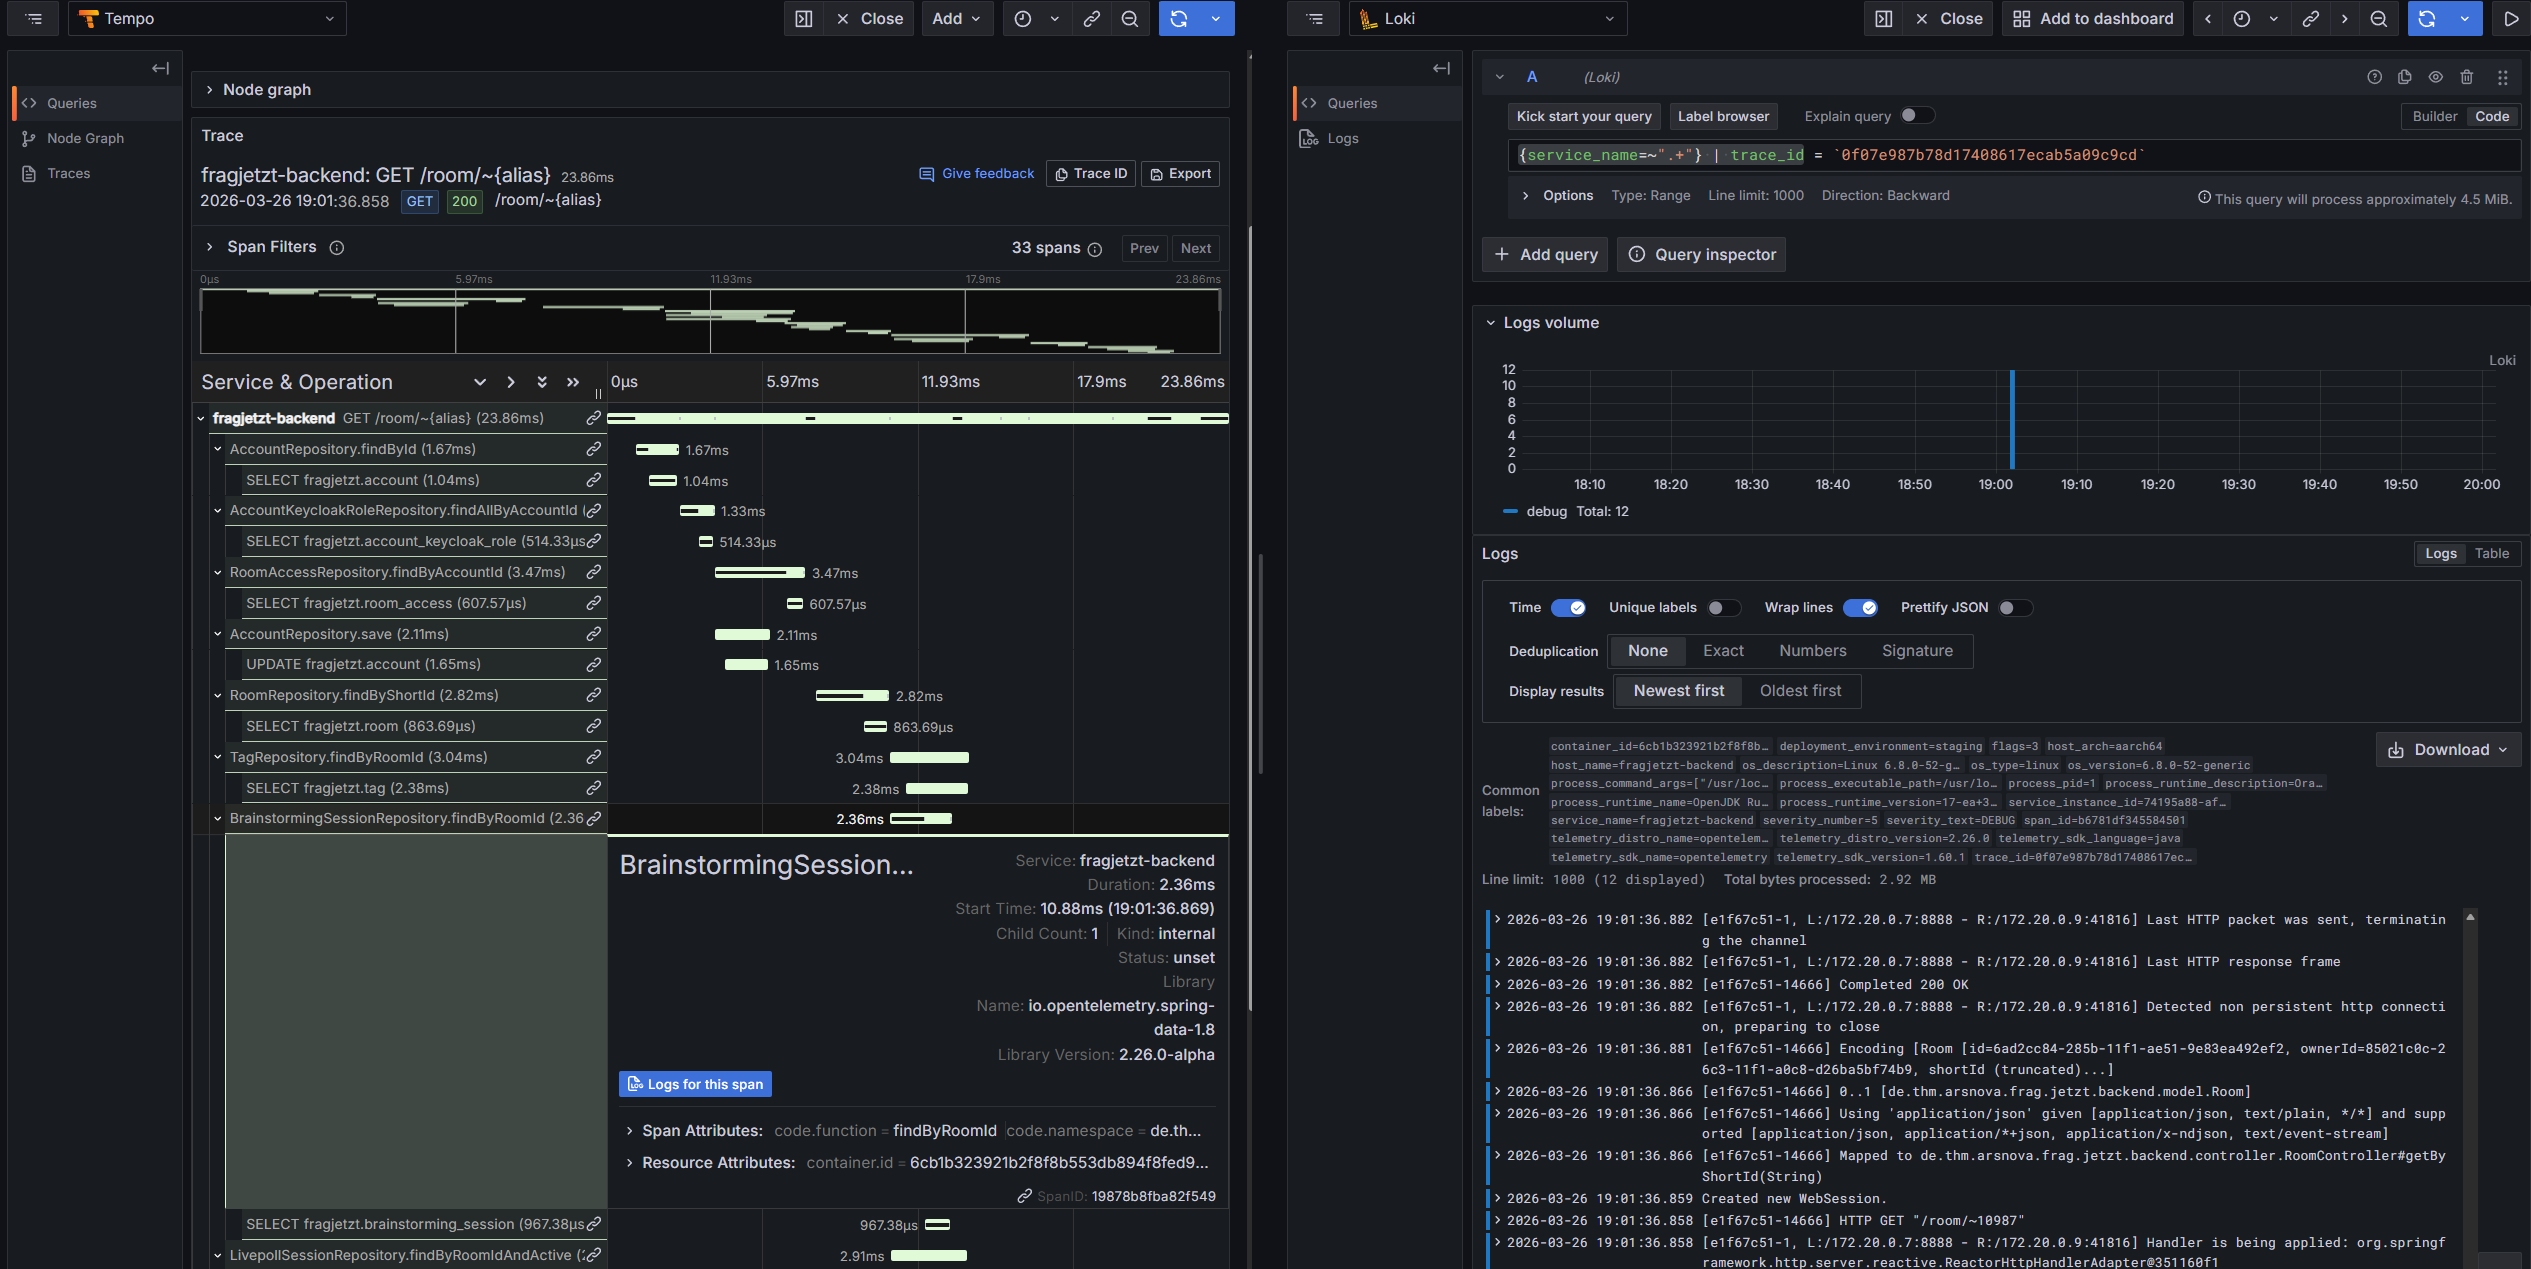
\includegraphics[width=\textwidth]{images/fig_trace_to_logs_correlation.png}
\caption[Trace-Waterfall in Tempo für den Endpunkt \texttt{GET /room/\{id\}/moderator} mit 11~Spans und zugeordneten Datenbankoperationen.]{Trace-Waterfall in Tempo für den Endpunkt \texttt{GET /room/\{id\}/moderator} mit 11~Spans und zugeordneten Datenbankoperationen. Der rechte Bereich zeigt die korrelierten Loki-Logs, erreichbar über die Funktion \emph{Logs for this span}. \small Quelle: Eigene Darstellung (Screenshot, Staging-Server).}
\label{fig:trace-waterfall}
\end{figure}

Die Nachvollziehbarkeit endet an den Grenzen der instrumentierten Komponenten. Der AI Provider und das Frontend sind nicht instrumentiert. Für den instrumentierten Backend-Pfad ist die Request-Rekonstruktion funktional gegeben, für das Gesamtsystem bleibt sie unvollständig. Der Erfüllungsgrad wird daher als \emph{teilweise erfüllt} bewertet.


\subsection{A2: Mehrstufige Messbarkeit entlang der Golden Signals}

\emph{Prüffrage: Deckt die Instrumentierung alle drei Messebenen ab?}

Das Golden-Signals-Dashboard bildet alle vier Dimensionen in separaten Sektionen ab. Im Belastungsszenario stieg die p95-Latenz unter CPU-Last von rund 20\,ms auf über 500\,ms, was im Dashboard sofort sichtbar wurde. Nach dem temporären Stopp der Datenbank stieg die 5xx-Rate und die betroffenen Endpunkte erschienen in der Fehlertabelle. Die drei Messebenen, Applikationsmetriken über den OTel Agent, Infrastrukturmetriken über Exporter und Trace-basierte Span-Metriken über Tempo, sind für die instrumentierten Dienste abgedeckt. Die Lücke betrifft die fehlende Frontend-Telemetrie. Der Erfüllungsgrad wird als \emph{weitgehend erfüllt} eingestuft.


\subsection{A3: Strukturiertes, korrelierbares Logging}

\emph{Prüffrage: Können Logeinträge über Korrelations-IDs verknüpft werden?}

Die bidirektionale Korrelation zwischen Logs und Traces konnte auf dem Staging-Server nachgewiesen werden. Von einem Trace in Tempo führt die Funktion \emph{Logs for this span} zu einer Loki-Abfrage, die nach Trace-ID und Dienstname filtert. In der Gegenrichtung enthält jeder Log-Eintrag in Loki ein klickbares \emph{TraceID}-Feld, das direkt zum zugehörigen Trace navigiert. Diese Verknüpfung wurde über ein Derived Field in der Loki-Datenquellenkonfiguration realisiert.

\begin{figure}[htb]
\centering
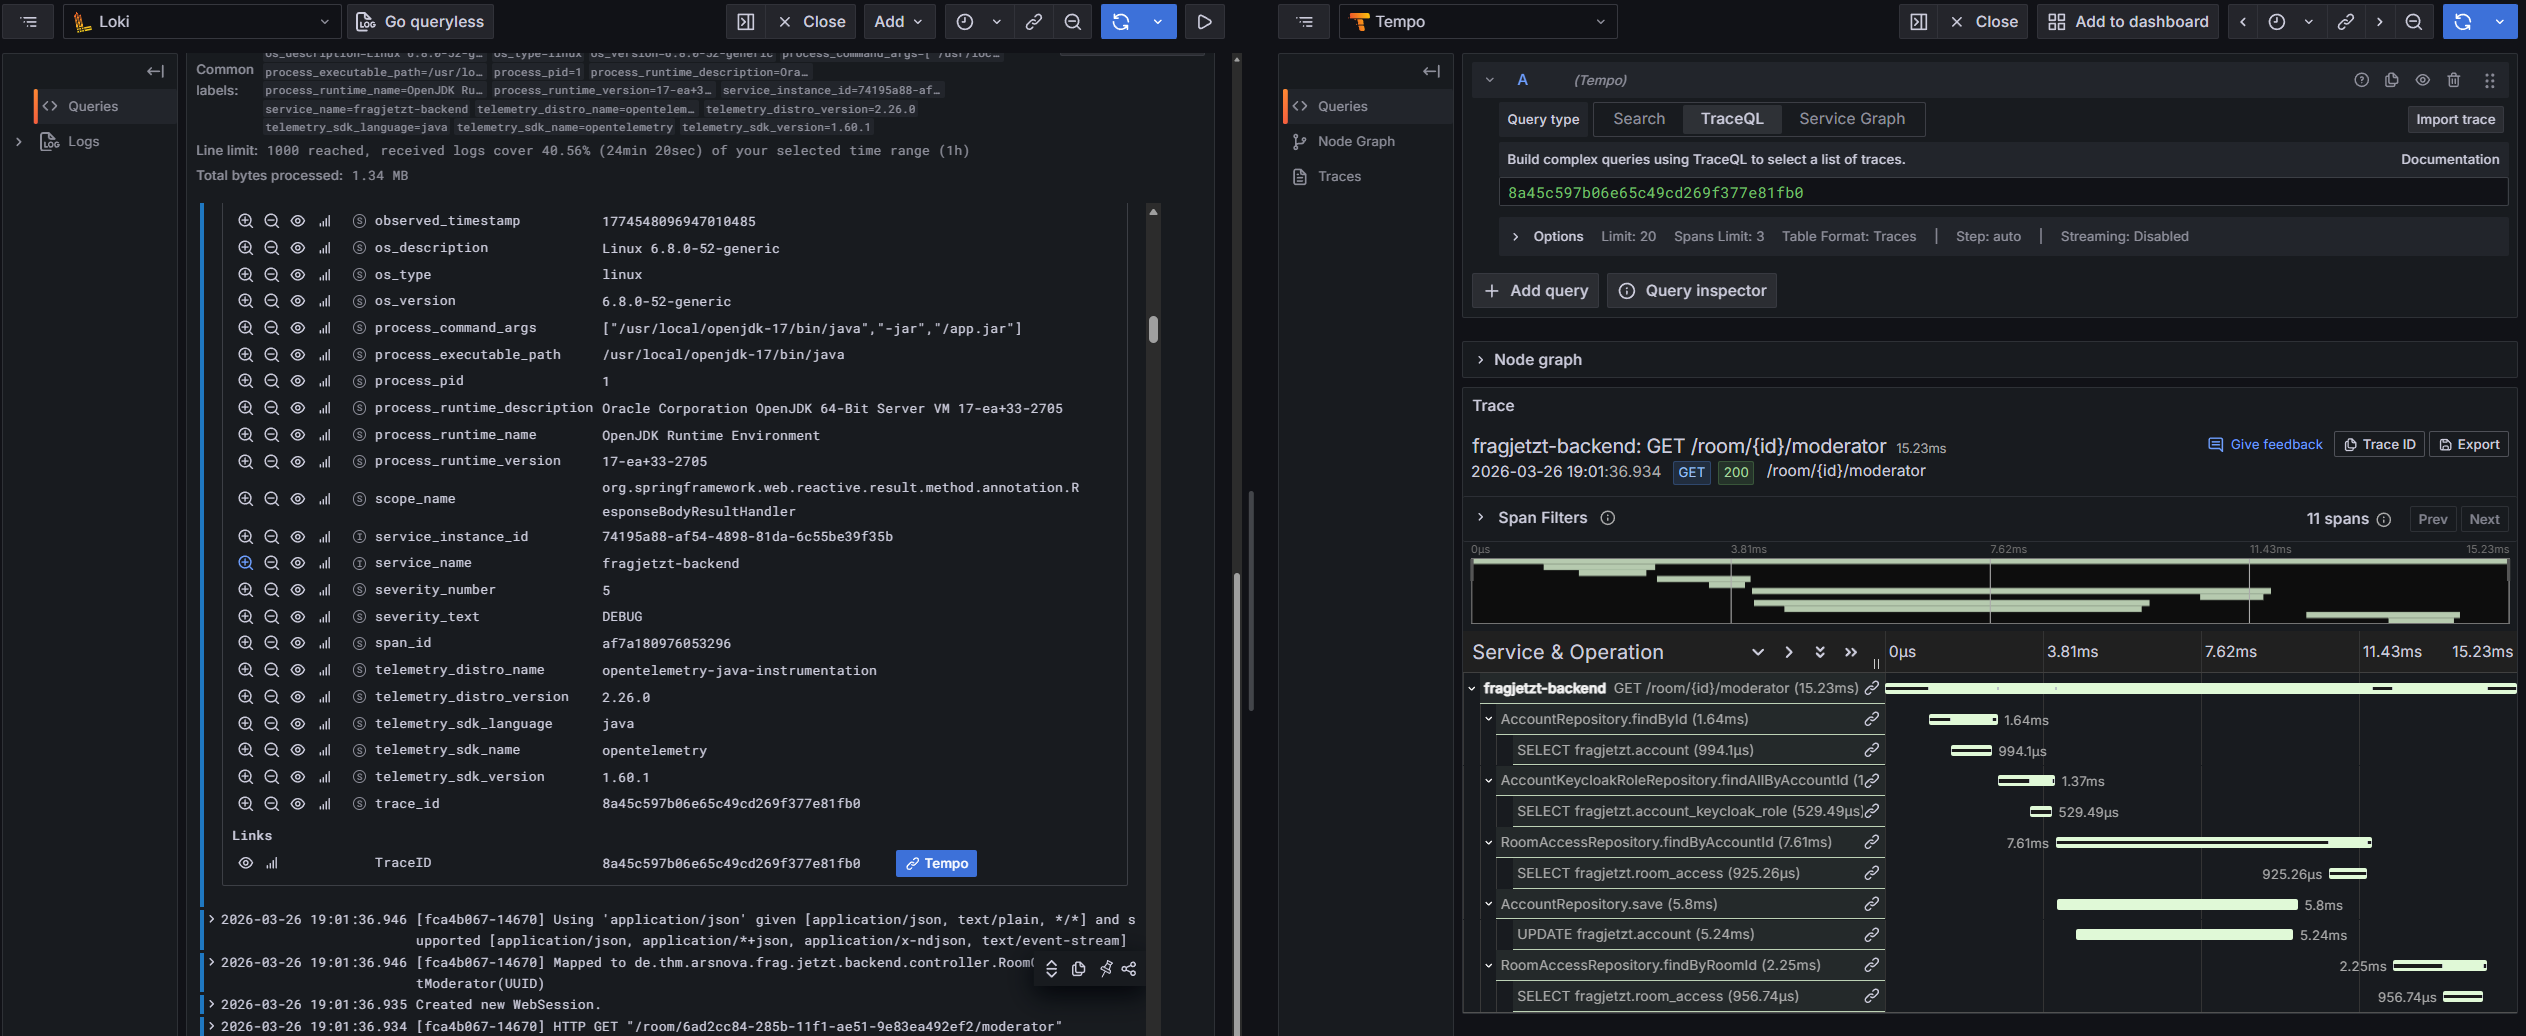
\includegraphics[width=\textwidth]{images/fig_log_to_trace_correlation.png}
\caption[Log-to-Trace-Korrelation in Loki: Ein Logeintrag mit klickbarem TraceID-Link (links) navigiert zum zugehörigen Trace-Waterfall in Tempo (rechts).]{Log-to-Trace-Korrelation in Loki: Ein Logeintrag mit klickbarem TraceID-Link (links) navigiert zum zugehörigen Trace-Waterfall in Tempo (rechts). \small Quelle: Eigene Darstellung (Screenshot, Staging-Server).}
\label{fig:log-to-trace}
\end{figure}

Da die Kernfunktion der Korrelierbarkeit nachgewiesen wurde, wird A3 als \emph{erfüllt} bewertet. Für den Produktivbetrieb wäre eine Reduktion auf strukturierte JSON-Protokollierung erforderlich.


\subsection{A4: Handlungsfähige Alarmierung}

\emph{Prüffrage: Reagieren Alarme auf nutzerwirksame Zustände und enthalten sie ausreichend Kontext für eine Erstreaktion?}

Der Latenz-Alert wurde durch künstlich erzeugten CPU-Druck auf den Backend-Container im Zustand \emph{Firing} ausgelöst. Abbildung~\ref{fig:alert-firing} zeigt den Alarm mit Symptombeschreibung, Prüfpfad und Runbook-Link in den Annotations. Die Multi-Signal-Logik bewährte sich: In Leerlaufphasen ohne aktive Requests verhinderte die Mindest-Traffic-Rate von 0,1\,req/s, dass der Alert fälschlicherweise auslöste.

\begin{figure}[htb]
\centering
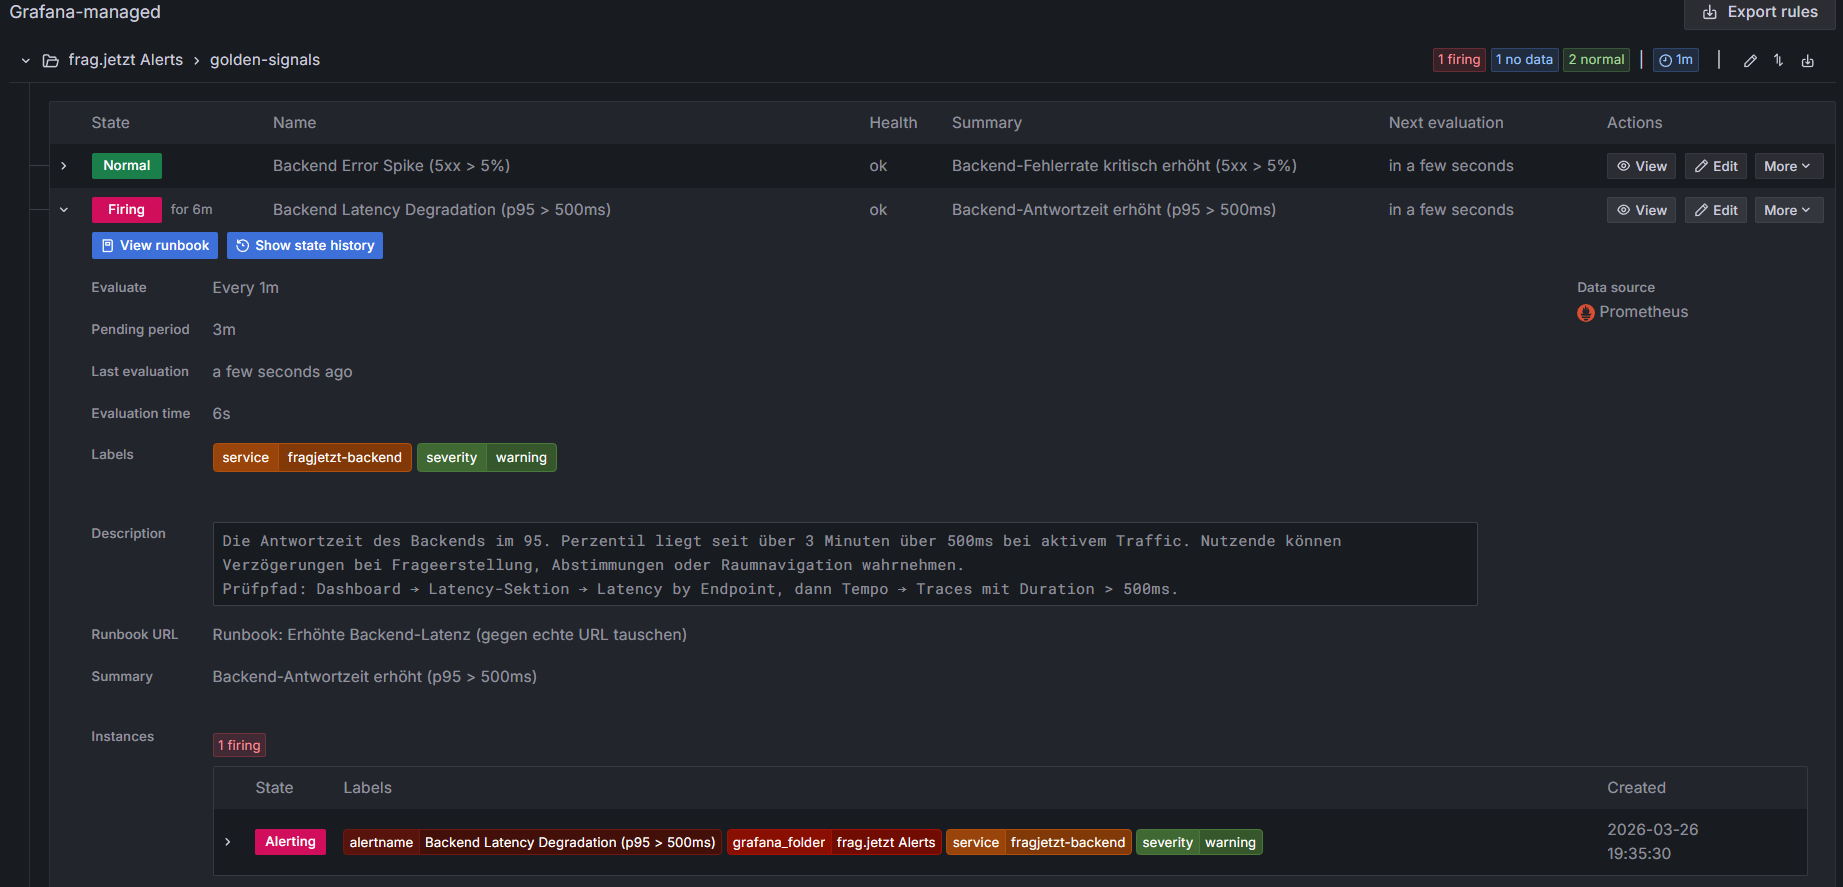
\includegraphics[width=\textwidth]{images/fig_firing_latency_alert.png}
\caption[Latenz-Alert im Zustand \emph{Firing} nach 6~Minuten. Die Annotations enthalten Symptombeschreibung, Prüfpfad und Runbook-Link.]{Latenz-Alert im Zustand \emph{Firing} nach 6~Minuten. Die Annotations enthalten Symptombeschreibung, Prüfpfad und Runbook-Link. \small Quelle: Eigene Darstellung (Screenshot, Staging-Server).}
\label{fig:alert-firing}
\end{figure}

Der Fehler-Alert konnte zuverlässig ausgelöst werden. Die Rate-Berechnung lieferte allerdings bei kurzen Betrachtungszeiträumen keine konsistenten Werte, vermutlich aufgrund einer Diskrepanz zwischen dem dynamisch berechneten Abfragefenster und der Erfassungssemantik der OTel-basierten Metriken. Der Sättigungs-Alert wurde nicht als eigenständiges Szenario getestet, die zugrunde liegende Metrik war jedoch korrekt verfügbar.

Für den Latenz-Alert ist die Alerting-Konzeption funktional validiert. Für den Fehler-Alert zeigt sich ein Datenqualitätsproblem in der kurzfristigen Metrikdarstellung, das die konzeptionelle Validität der Regel nicht infrage stellt, aber die operative Kurzfristdiagnose einschränkt. Der Erfüllungsgrad wird als \emph{teilweise erfüllt} eingestuft.


\subsection{A5: Beobachtbarkeit der Infrastrukturschicht}

\emph{Prüffrage: Werden Container-Ressourcen, Datenbankpool-Auslastung und Queue-Tiefen erfasst?}

Die Infrastruktur-Sektion des Dashboards beantwortet diese Frage positiv. Abbildung~\ref{fig:infrastructure-dashboard} zeigt PostgreSQL-Verbindungszähler, RabbitMQ-Queue-Tiefen, Host-Ressourcen und den Service Graph. Während der Belastungstests stieg die Zahl aktiver PostgreSQL-Verbindungen von einem Normalniveau um 3 auf temporär über 10. Alle fünf Infrastruktur-Exporter lieferten während des gesamten Evaluationszeitraums durchgängig Metriken. Da die Metriken verfügbar und plausibel sind, nicht aber alle Indikatoren unter gezielter Last geprüft wurden, wird A5 als \emph{weitgehend erfüllt} bewertet.

\begin{figure}[htb]
\centering
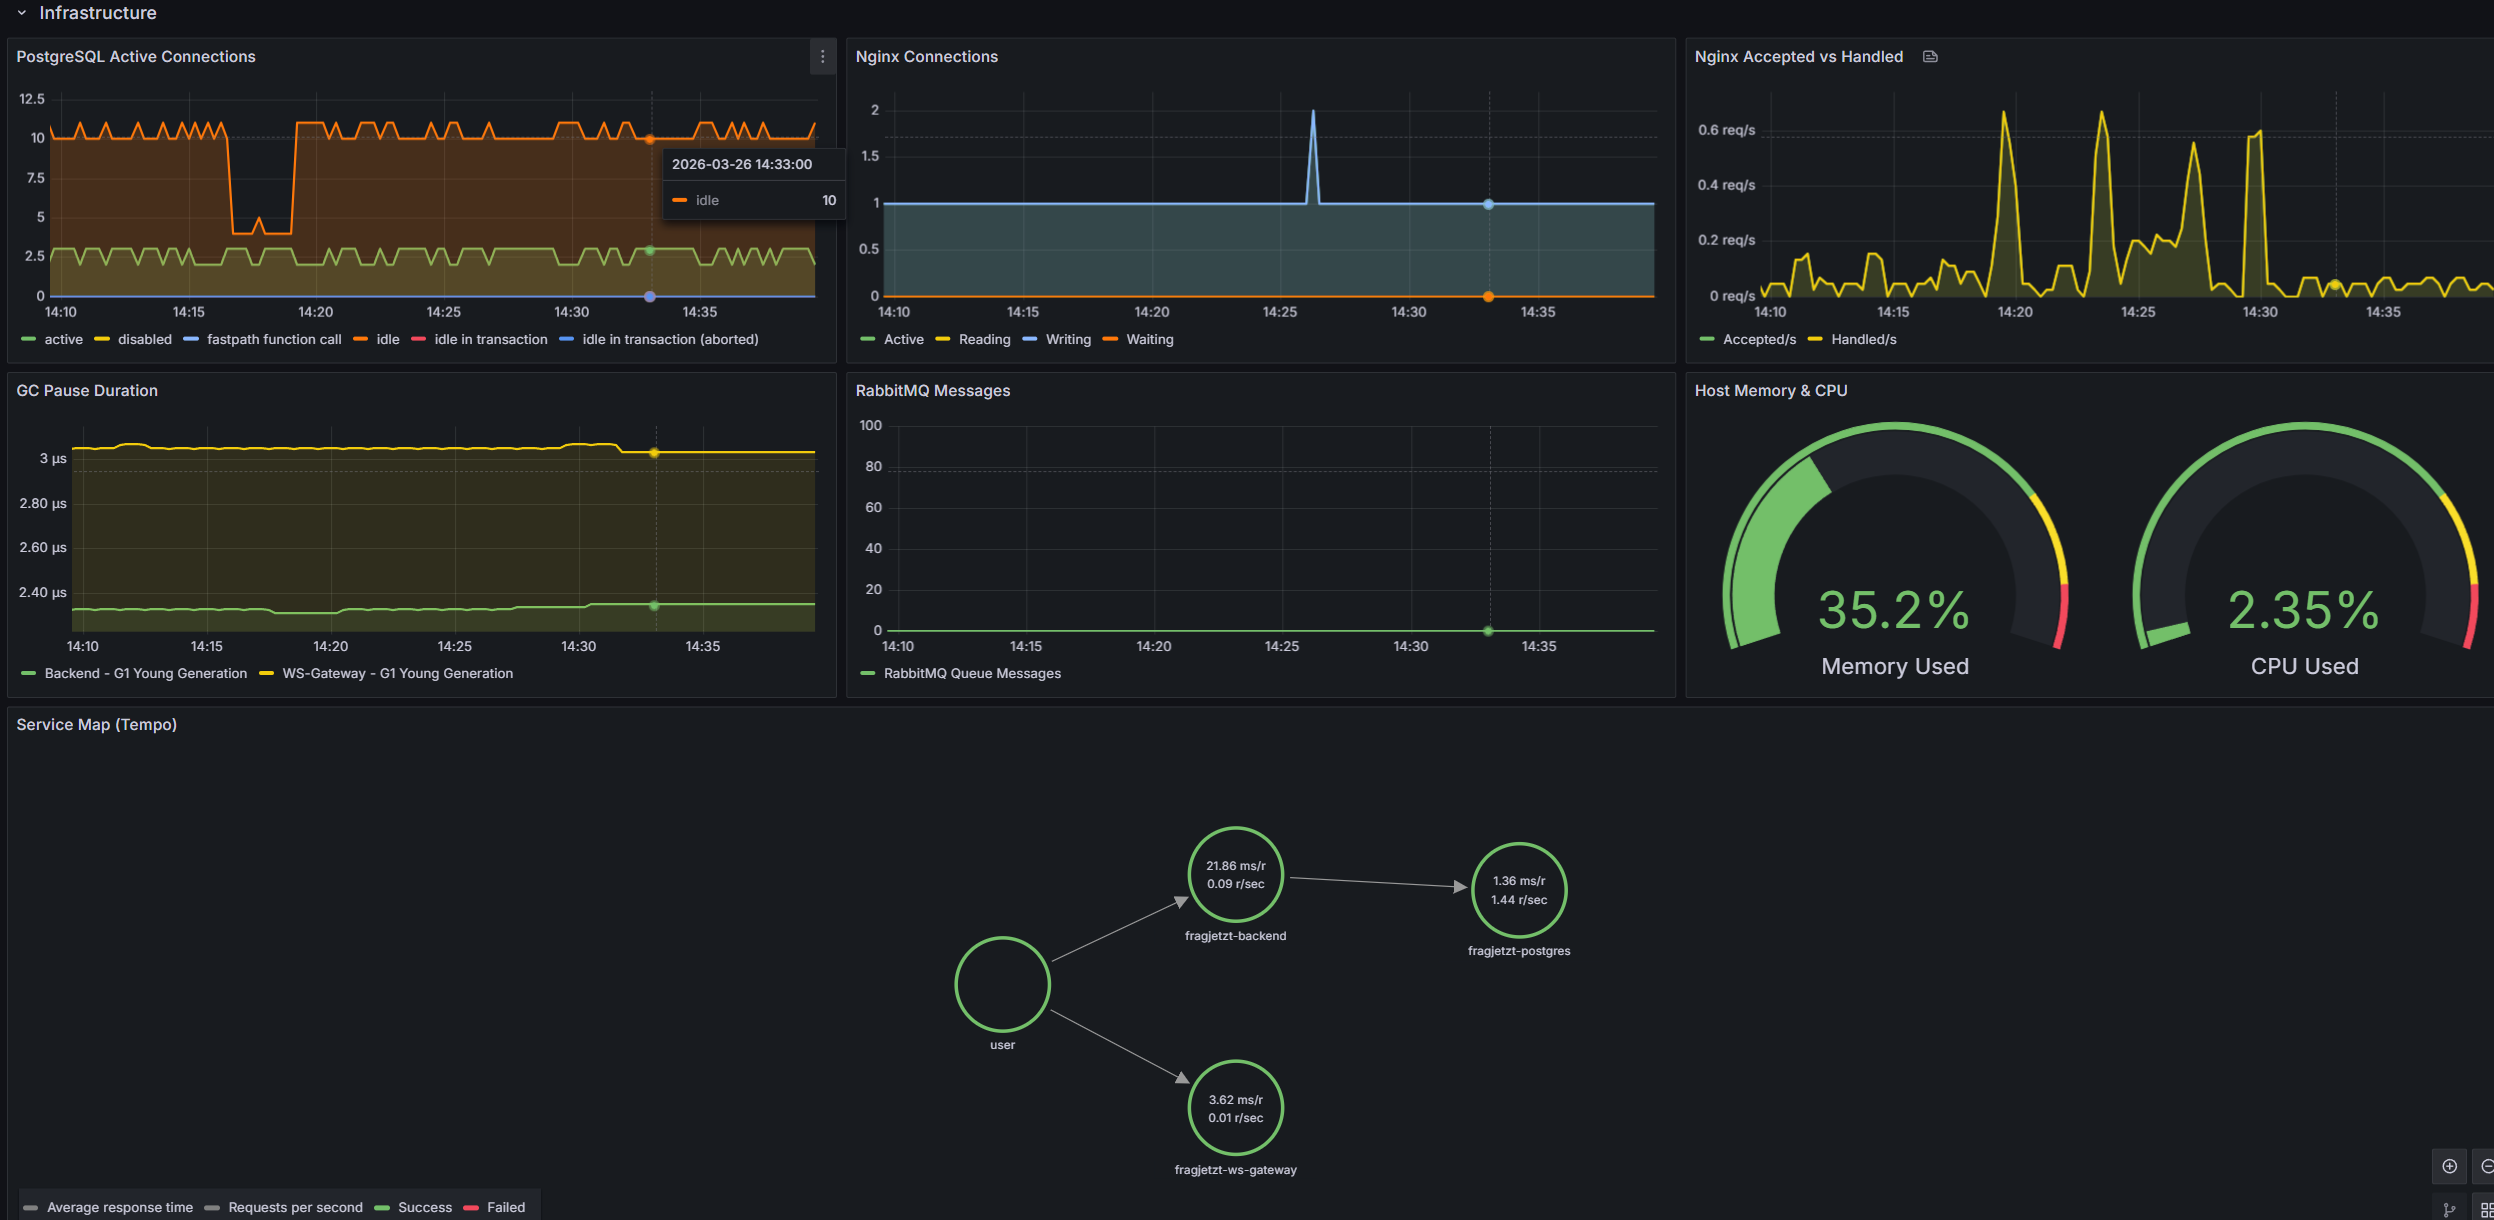
\includegraphics[width=\textwidth]{images/Grafana-Dashboard_Infrastructure.png}
\caption[Infrastruktur-Sektion des Golden-Signals-Dashboards mit PostgreSQL-Verbindungen, RabbitMQ-Queue-Tiefe, Host-Ressourcen und Service Graph.]{Infrastruktur-Sektion des Golden-Signals-Dashboards mit PostgreSQL-Verbindungen, RabbitMQ-Queue-Tiefe, Host-Ressourcen und Service Graph. \small Quelle: Eigene Darstellung (Screenshot, Staging-Server).}
\label{fig:infrastructure-dashboard}
\end{figure}


\section{Übergreifende Bewertungsdimensionen}

\paragraph{Stakeholder-Tauglichkeit.}
Für die DevOps-Perspektive ist der Prototyp funktional nutzbar: Dashboard, Alerting-Regeln und Runbooks liefern eine zusammenhängende Diagnoseinfrastruktur. Für die Entwicklungsperspektive ermöglicht Grafana Explore die direkte Abfrage von Traces, Logs und Metriken mit bidirektionaler Korrelation, ein dediziertes Entwickler-Dashboard wurde jedoch nicht umgesetzt. Für die Product-Owner-Perspektive fehlt im Prototyp eine eigene Sicht, die technisch aus den vorhandenen Datenquellen ableitbar wäre.

\paragraph{Abdeckung der Risikopunkte.}
Von den sechs identifizierten Risikopunkten werden R2 (DB-Contention), R3 (Intransparenz ohne Tracing) und R5 (Ressourcenverdrängung) durch den Prototyp direkt adressiert. R3 wurde durch die Einführung von Distributed Tracing beseitigt. R1 (fehlende Timeouts) und R4 (Backend als Single Point of Failure) bleiben als architektonische Defizite bestehen, die über Beobachtbarkeit sichtbar, aber nicht lösbar sind.

\paragraph{Umsetzungsrealismus.}
Die Gesamtdauer von der initialen Stack-Konfiguration bis zum funktionierenden Dashboard betrug wenige Arbeitstage. Der laufende Betrieb des Observability-Stacks erfordert allerdings ein eigenes Ressourcenbudget, das bei der Kapazitätsplanung des Hosts berücksichtigt werden muss.


\section{Grenzen und methodische Einschränkungen}

Die Evaluation unterliegt fünf Einschränkungen.

\emph{Erstens, unvollständige Dienstabdeckung.} Backend und WS-Gateway sind instrumentiert, AI Provider und Frontend nicht. Die Bewertung von A1 und A2 gilt nur für einen Teil des Gesamtsystems.

\emph{Zweitens, Stabilität des Observability-Stacks unter Last.} Tempo wurde während der Belastungstests durch Speichererschöpfung beendet (OOM-Kill), woraufhin auch der OTel Collector den Betrieb einstellte. Infrastrukturmetriken über die Prometheus-Exporter blieben unberührt. Der Vorfall verdeutlicht, dass der Observability-Stack selbst eine Fehlerquelle darstellt, deren Auswirkungen auf einem Single-Host-System die Beobachtbarkeit des Gesamtsystems beeinträchtigen.

\emph{Drittens, eingeschränkte Aussagekraft der Rate-Berechnung.} Die PromQL-Variable \texttt{\$\_\_rate\_interval} lieferte bei kurzen Betrachtungszeiträumen inkonsistente Ergebnisse für die HTTP-5xx-Rate. In längeren Zeitfenstern (ab circa 12~Stunden) waren die Werte korrekt. Diese Einschränkung betrifft die Dashboard-Darstellung, nicht die Alerting-Regeln mit festen Zeitfenstern.

\emph{Viertens, fehlende Produktivdaten.} Alle Tests wurden mit synthetischer Last durchgeführt. Reale Nutzungsmuster, insbesondere die Lastspitzen während Lehrveranstaltungen, konnten nicht abgebildet werden. Die Schwellenwerte müssten im Produktivbetrieb anhand realer Lastprofile kalibriert werden.

\emph{Fünftens, prototypische Testmethodik.} Die Belastungsszenarien wurden manuell über Konsolen-Schleifen und Container-Operationen durchgeführt. Für eine belastbarere Validierung wäre ein dedizierter HTTP-Lastgenerator mit kontrollierten Lastprofilen erforderlich.